\section{Zadania projektowe i plan
pracy}\label{zadania-projektowe-i-plan-pracy}

\textbf{Zadanie:} \textbf{Zebranie danych} \textbf{Skrótowa nazwa:}
Zebranie danych\\\textbf{Czas realizacji:} 16.03 - 30.03\\\textbf{Opis:}
Identyfikacja i ocena dostępnych źródeł danych, wstępna analiza ich
przydatności i zawartości.\\\textbf{Produkty:} Artefaktem
potwierdzającym ukończenie zadania i zawierającym rezultaty
przeprowadzonych działań będzie dokument ``Analiza źródeł danych''

\textbf{Zadanie:} \textbf{Wybór atrybutów} \textbf{Skrótowa nazwa:}
Wybór atrybutów\\\textbf{Czas realizacji:} 30.03 - 13.04\\\textbf{Opis:}
Dogłębna analiza danych zawartych w źródłach i wybór kryteriów przyszłej
analizy oraz selekcja tych atrybutów ze źródeł, które będą konieczne do
realizacji celów projektowych.\\\textbf{Produkty:} Artefaktem z tego
zadania będzie dokument ``Kryteria analizy''

\textbf{Zadanie:} \textbf{Opracowanie wspólnego formatu danych i
schematu bazy}\\\textbf{Skrótowa nazwa:} Wspólny format\\\textbf{Czas
realizacji:} 06.04 - 20.04\\\textbf{Opis:} Stworzenie zgodnie z dokonaną
wcześniej selekcją atrybutów wspólnego formatu danych. Obejmuje zarówno
ujednolicenie formatu danych (np. data, sposób oznaczenia miejsca
wypadku) jak i semantyki (np. obranie wspólnych określeń na warunki
atmosferyczne panujące w momencie wypadku).\\\textbf{Produkty:} W
związku z tym zadaniem powstaną następujące artefakty: dokument
``Projekt bazy danych'' zawierający opis formatu i semantyki danych oraz
schemat bazy danych.

\textbf{Zadanie:} \textbf{Integracja danych i zapis do
bazy}\\\textbf{Skrótowa nazwa:} Integracja\\\textbf{Czas realizacji:}
13.04 - 04.05\\\textbf{Opis:} Ekstrakcja danych ze źródeł, transformacja
do wspólnego formatu i załadowanie do bazy danych. Obejmuje utworzenie
skryptów parsujących i konwertujących na wspólny format i wspólną
semantykę.\\\textbf{Produkty:} Produktami tego zadania będą skrypty oraz
uzupełniona baza danych.

\textbf{Zadanie:} \textbf{Statystyczna analiza danych}\\\textbf{Skrótowa
nazwa:} Analiza statystyczna\\\textbf{Czas realizacji:} 04.05 -
25.05\\\textbf{Opis:} Statystyczna analiza danych w celu wyłonienia
możliwych przyczyn wypadku, zgodna z określonymi wcześniej
kryteriami.\\\textbf{Produkty:} Realizacja tego zadania przejawi się w
następujących produktach: skrypty przeprowadzające analizy, wykresy
obrazujące przeprowadzone analizy, dokument ``Raport z analiz'', który
będzie tworzony stopniowo, być może jako zbiór mniejszych dokumentów
wraz z przeprowadzaniem kolejnych analiz oraz dokument ``Wnioski z
analiz'', który będzie opisywał wnioski na temat przyczyn wypadków
drogowych wyciągnięte na podstawie przeprowadzonych analiz.

\textbf{Zadanie:} \textbf{Zaawansowana analiza danych}\\\textbf{Skrótowa
nazwa:} Zaawansowana analiza\\\textbf{Czas realizacji:} 18.05 -
8.06\\\textbf{Opis:} Zaawansowana analiza danych w celu wyłonienia
możliwych przyczyn wypadku, korzystająca z mechanizmów takich jak
klasteryzacja czy wyszukiwanie wzorców częstych.\\\textbf{Produkty:}
Realizacja tego zadania przejawi się w następujących produktach: skrypty
przeprowadzające analizy, wykresy obrazujące przeprowadzone analizy,
dalsze części dokumentu ``Raport z analiz'', oraz dalsze części
dokumentu ``Wnioski z analiz'' (patrz zadanie Statystyczna analiza
danych).

\section{Wykres Gantta}\label{wykres-gantta}

Opisane powyżej zadania zostały przedstawione na wykresie Gantta,
zgodnie z przewidywanymi terminami ich wykonywania.

\begin{figure}[htbp]
\centering
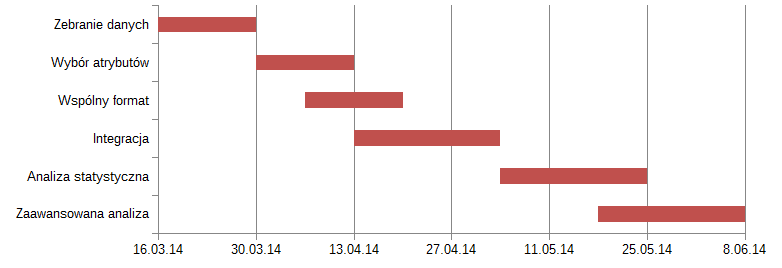
\includegraphics[width=0.9\textwidth]{images/gantt.png}
\caption{Diagram Gantta}
\end{figure}

\section{Ryzyko w projekcie}\label{ryzyko-w-projekcie}

Prawdopodobieństwo wystąpienia oraz wpływ na projekt podane w skali 1-5

\textbf{Ryzyko:} Problem z uzyskaniem części danych\\\textbf{Opis:}
Otrzymanie danych z POBR jest uzależnione od fizycznej osoby, która musi
przydzielić możliwość pełnego dostępu do danych po wcześniejszym
otrzymaniu stosownego pisma. Procedura taka może za długo trwać i nie
zdążymy uwzględnić tych danych w projekcie.\\\textbf{Prawdopodobieństwo
wystąpienia:} 4\\\textbf{Wpływ na projekt:} 2\\\textbf{Rozwiązanie:}
Praca z danymi dostępnymi i uwzględnienie niedostępnych danych w postaci
statystyk

\textbf{Ryzyko:} Problem z ustaleniem wspólnego formatu
danych\\\textbf{Opis:} Dane, z których korzystamy, pochodzą z bardzo
różnych źródeł, mają różną semantykę i format. Może się okazać niezwykle
trudne stworzenie wspólnego formatu danych dla tych źródeł, które
jednocześnie będzie maksymalnie wykorzystywał dane w nich
dostępne\\\textbf{Prawdopodobieństwo wystąpienia:} 4\\\textbf{Wpływ na
projekt:} 4\\\textbf{Rozwiązanie:} W razie konieczności zawężenie
wspólnego formatu danych i w konsekwencji utrata części danych z
niektórych źródeł

\textbf{Ryzyko:} Duża ilość brakujących danych\\\textbf{Opis:} Wiele
przydatnych informacji może brakować dla części danych. Część ta może
się okazać bardzo duża\\\textbf{Prawdopodobieństwo wystąpienia:}
3\\\textbf{Wpływ na projekt:} 2\\\textbf{Rozwiązanie:} Problem
brakujących danych jest trudny do zwalczenia, gdyż nie ma możliwości
uzupełnienia ich wszystkich, należy więc w taki sposób zaprojektować
analizy aby uwzględnić możliwość braku niektórych danych.

\textbf{Ryzyko:} Duża ilość danych\\\textbf{Opis:} Źródła danych, z
którymi będziemy pracować w projekcie zawierają dużo
danych.\\\textbf{Prawdopodobieństwo wystąpienia:} 4\\\textbf{Wpływ na
projekt:} 2\\\textbf{Rozwiązanie:} Duża ilość danych jest z jednej
strony dobra gdyż pozwala stwierdzić reprezentatywność analiz i rozważyć
wiele przypadków, może być jednak kłopotliwa w przeprowadzaniu analiz.
Należy dobrze zaprojektować bazę danych i ograniczyć się do
przechowywania tych atrybutów, które będą naprawdę przydatne w analizie.
Analizy musza brać pod uwagę ilość danych i np. ograniczać się do
analizowania w danym momencie danych z jednego roku.
